\section{Dataset and demand model}
\label{sec:10_3_dataset}

%****************************************
% Motivation and outline
%****************************************
In this work we leverage the data collected in our previous work~\cite{10_ciociola2017umap} capturing real trips performed by car2go users. These data let us model the users' mobility demand in time and in space. From this, we derive a demand model that generalize the users' demand observed in the real data. We use it to generate realistic traces describing possible user trips and feed them to our event-based simulator to derive performance figures.

%****************************************
% Details of dataset and characterization
%****************************************

\begin{figure}
    \begin{center}
            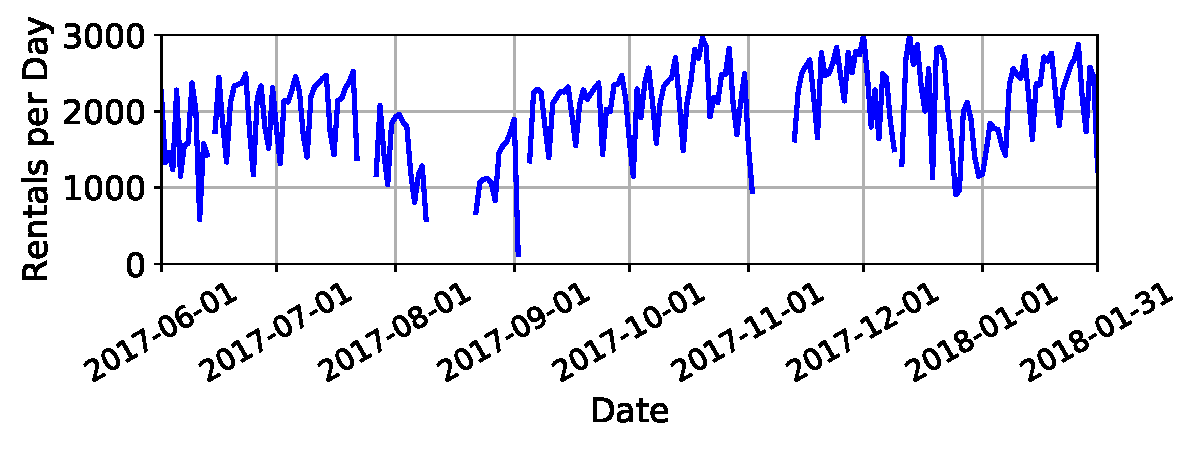
\includegraphics[width=\columnwidth]{fig/RentalsDay.pdf}
            \caption{Number of rentals per day in Turin, from June 2017 to January 2018. Some data is missing.}
            \label{fig:10_3_rentals_per_day}
            \end{center}
\end{figure}


\subsection{Dataset}

Our data consist in actual rentals performed by car2go users in Turin. Each observed rental has precise geo-spatial coordinates for trip origin and destination, and accurate timestamps. In Figure~\ref{fig:10_3_rentals_per_day} we summarize the number of daily rentals from June 2017 to January 2018 in Turin, our reference dataset\footnote{For some periods we did not record data due to server failures.}.  Despite the fact that rentals are non-stationary, especially during periods like August and Christmas holidays, the service usage follows a hourly and weekly pattern, not showing any particular growth. From this data, we select three months - from October 1st to December 31st.
Table~\ref{tab:10_3_rental_data} outlines the main characteristics of this data. 400 cars were available, traveling on average less than 4\,km in each trip, for an average rental time of 21 minutes.


To catch customers' habits, in Figure~\ref{fig:10_3_rentals_per_hour} we detail the average number of rentals per hour, separately per working-days (Monday to Friday) and per weekends. The weekdays hourly profile reflects the commuting pattern, with two clear peaks in the morning and evening rush hours. Conversely, during the weekends the number of night rentals is higher, likely due to more nightlife, while the morning peak is drastically smoothed.
Not shown here for lack of space, our data allow us to observe the spatial diversity, with different origin and destination areas over the city. This shows how fundamental is to use actual data to build realistic scenarios for accurate system analysis.



\begin{table}[t]
\begin{center}
\setlength\tabcolsep{5pt} % default value: 6pt reduce cell padding
\caption{Main characteristics of our dataset, recorded in Turin from October to December 2017. Rental time and rental distance report both median (Med) and average (Avg) values.}
\begin{tabular}{|l|l|l|c|c|c|l|}
\hline
\!\multirow{3}{*}{Rentals}\!& \multirow{2}{*}{Fleet} &  \multicolumn{2}{|c|}{Rental}  &  \multicolumn{2}{|c|}{Rental}  &  \!\multirow{3}{*}{Zones}\!\\ 
& \multirow{2}{*}{Size}  & \multicolumn{2}{|c|}{Time~[min]}  & \multicolumn{2}{|c|}{Dist.~[km]} &    \\ \cline{3-6} %&  \multirow{2}{*}{Size[GB]}
 &  &\!Avg\!&\!Med\!&\!Avg\!&\!Med\!& \\ \hline
\hline
 180k & 400 & 21 & 20 & 3.96 & 3.36 & 279 \\ \hline
\end{tabular}
\label{tab:10_3_rental_data}
\end{center}
\end{table}


\begin{figure}[t]
    \begin{center}
             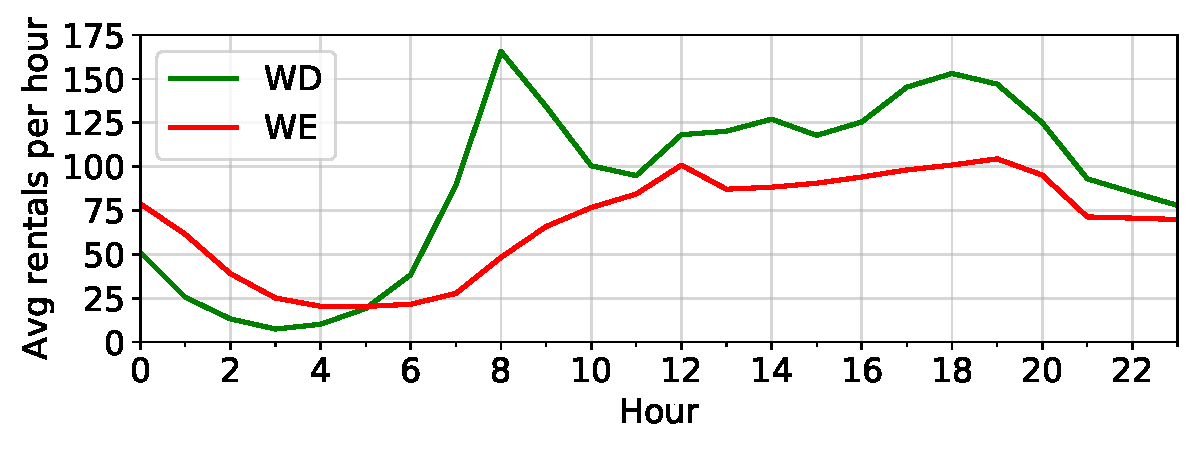
\includegraphics[width=\columnwidth]{fig/RentalsHour.pdf}
             \caption{Average number of rentals per hour during weekdays (WD) and weekends (WE). }
             \label{fig:10_3_rentals_per_hour}
            \end{center}
\end{figure}



%****************************************
% Demand model
%****************************************
\subsection{Demand Model}
 
While we could directly use the original trace to observe system performance, we need a model to observe what-if scenarios, e.g., to observe the impact of a growth in the demand. For this, we use the data at our disposal to create a generalized demand model. We follow the approach we presented in~\cite{ciociola2020}. In a nutshell we model the demand in time by using modulated Poisson processes - a common accepted model for independent service requests of a very large population~\cite{poisson_inh}. To capture the spatial heterogeneity, we generalize the traces using Kernel Density Estimation (KDE)~\cite{kde_spatial}. KDE gives us the possibility to smooth the real data over a multi-dimensional space while maintaining the origin/destination correlation.
%%%%%%%%%%%%%%%%%%%%%%%%%%%%%%%%%%%%%%%%%%%%
%Model of departure times
%%%%%%%%%%%%%%%%%%%%%%%%%%%%%%%%%%%%%%%%%%%%%
In more details, for the request arrival time process we assume that the inter-arrival time of trips follows an exponential distribution with rate depending on the type (weekend or working day) and hour of the day. We consider 24 time bins of 1\,h each - 48 periods in total. In each time/day bin, the Poisson arrival rate matches the average rate of requests in that time bin in the original dataset as shown in Figure~\ref{fig:rentals_per_hour}. This temporal model allows to scale the overall demand by introducing a global scaling factor $\lambda$ as a multiplier of the request rate of each time bin.

To model the spatial diversity of the demand, we divide the city in a set $Z$ of contiguous 500\,m x 500\,m zones, obtaining in total 279 zones. Each couple of spatial coordinates in the city area  ($x,y$) maps to one and only one zone.  Since each trip $i$ departs from a certain zone (origin $O_i$, described by two coordinates) and arrives to another zone (destination $D_j$, described by two coordinates), it is therefore characterized by two couples of coordinates, that can be represented as 4 scalars. 
For each time bin, we derive an origin and destination matrix counting how many trips were originated from a given zone $O$ and destined to a given zone $D$. Thus, in order to model the OD matrix in each temporal slot, we fit a 4-dimensional KDE based on the aforesaid coordinates.
For each of these matrices, we compute a KDE model, using Gaussian kernels, with bandwidth equal to 1. % , i.e., concentrating 66\% of the body of the distribution  in the same 500\,m x 500\,m zone. \mm{controllare che sia corretto} \lv{e' piu' complicato di cosi'...} 
Not reported here for the sake of brevity, we compare the  number of trips generated from the model and the ones presented in the original trace. As expected, there is a very good match with low residuals. We refer the reader to~\cite{ciociola2020} for details.

Notice that we employ a single global scaling factor $\lambda$ directly the temporal model to keep the spatial distribution of trips unchanged while increasing the request rate. 